% ============================================================
%  RELATÓRIO — ARQUITETURAS DE ALTO DESEMPENHO
%  Prática 5: Filtro de Máximo/Mínimo em FPGA para
%             Processamento de Imagens Binárias com Saída VGA
%  Normas para Elaboração de Relatórios ver 4 (2026)
%  Universidade Federal de São Carlos (UFSCar)
% ============================================================
\documentclass[12pt, a4paper]{article}

% --- Codificação e idioma ---
\usepackage[utf8]{inputenc}
\usepackage[T1]{fontenc}
\usepackage[brazil]{babel}
\usepackage{amsmath}
\usepackage{amssymb}
\usepackage{multirow}

% --- Fonte Times New Roman ---
\usepackage{mathptmx}

% --- Geometria da página ---
\usepackage[
top=2.5cm,
bottom=2.5cm,
left=3.0cm,
right=3.0cm
]{geometry}

% --- Espaçamento entre linhas ---
\usepackage{setspace}
\onehalfspacing

% --- Indentação do parágrafo ---
\usepackage{indentfirst}
\setlength{\parindent}{1.25cm}

% --- Pacotes gráficos e de figuras ---
\usepackage{graphicx}
\usepackage{float}

% --- Tabelas ---
\usepackage{booktabs}
\usepackage{array}
\usepackage{longtable}

% --- Listagens de código ---
\usepackage{listings}
\usepackage{xcolor}

\lstdefinestyle{verilog}{
	language=Verilog,
	basicstyle=\ttfamily\small,
	keywordstyle=\color{blue}\bfseries,
	commentstyle=\color{gray}\itshape,
	stringstyle=\color{teal},
	numbers=left,
	numberstyle=\tiny\color{gray},
	stepnumber=1,
	numbersep=8pt,
	frame=single,
	breaklines=true,
	breakatwhitespace=true,
	columns=flexible,
	keepspaces=true,
	captionpos=b,
	morekeywords={module,endmodule,input,output,reg,wire,always,begin,end,
		posedge,negedge,if,else,case,endcase,assign,parameter,
		localparam,integer,initial,for,while,defparam}
}

% --- Numeração de seções ---
\setcounter{secnumdepth}{3}

% --- Cabeçalho e rodapé ---
\usepackage{fancyhdr}
\setlength{\headheight}{14pt}
\pagestyle{fancy}
\fancyhf{}
\fancyhead[R]{\small Arquiteturas de Alto Desempenho --- Relatório}
\fancyfoot[C]{\thepage}
\renewcommand{\headrulewidth}{0.4pt}

% --- Hiperlinks (DEVE ser o último pacote) ---
\usepackage[hidelinks]{hyperref}

% ============================================================
%  INÍCIO DO DOCUMENTO
% ============================================================
\begin{document}
	
	\thispagestyle{empty}
	
	% ============================================================
	%  CAPA
	% ============================================================
	\begin{titlepage}
		\centering
		
		\noindent\rule{\textwidth}{0.8pt}\\[0.2cm]
		{\large \textbf{UNIVERSIDADE FEDERAL DE SÃO CARLOS}}\\[0.15cm]
		{\normalsize Centro de Ciências Exatas e Tecnologia}\\[0.15cm]
		{\normalsize Departamento de Computação}\\[0.15cm]
		
		\vspace{0pt plus 0.35fill}
		
		{\large \textbf{Laboratório de Arquiteturas de Alto Desempenho}}\\[0.4cm]
		{\large Prática 5 --- Filtro de Máximo/Mínimo em FPGA para\\[0.2cm]
			Processamento de Imagens Binárias com Saída VGA}\\[1.0cm]
		{\normalsize Professor: \textit{Dr. Emerson Carlos Pedrino}}\\
		
		\vspace{0pt plus 0.65fill}
		
		\begin{center}
			{\normalsize \textit{Pedro Augusto Faria} \ (RA: \textit{821124})}\\[0.15cm]
			{\normalsize Curso: \textit{Engenharia da Computação}}\\[0.15cm]
		\end{center}
		
	\end{titlepage}
	
	\setcounter{page}{1}
	
	% ============================================================
	%  SEÇÃO 1 — INTRODUÇÃO
	% ============================================================
	\section{Introdução}
	
	O processamento de imagens em hardware reconfigurável constitui um dos campos
	mais relevantes das arquiteturas de alto desempenho. Diferentemente de soluções
	baseadas em software, onde um processador de propósito geral executa instruções
	sequencialmente, a implementação direta em FPGA (\textit{Field-Programmable Gate
		Array}) permite explorar paralelismo espacial intrínseco ao problema: múltiplas
	operações sobre pixels distintos ocorrem simultaneamente em hardware dedicado,
	ao custo de um único ciclo de clock.
	
	Esta prática aborda a construção de um sistema completo de processamento de imagens
	binárias na placa Altera DE1 (Cyclone V), utilizando o ambiente Quartus Prime.
	O sistema recebe uma imagem binária ruidosa de 256$\times$128 pixels armazenada
	em memória ROM, aplica filtragem morfológica por meio de um pipeline de estágios
	encadeados, e exibe tanto a imagem original quanto a processada em um monitor VGA
	de resolução 640$\times$480 pixels, mediante seleção por chaves (\textit{switches})
	da placa.
	
	O ruído do tipo \textit{sal e pimenta} é um dos artefatos mais comuns em sistemas
	de aquisição de imagens binárias. Ele se manifesta como pixels brancos espúrios em
	regiões escuras (\textit{sal}) e pixels pretos espúrios em regiões claras
	(\textit{pimenta}), distribuídos de forma aleatória e independente. Sua presença
	degrada substancialmente a qualidade de etapas subsequentes de análise --- como
	segmentação, reconhecimento de formas ou contagem de objetos --- tornando a
	filtragem um pré-processamento indispensável.
	
	A solução adotada emprega operações morfológicas binárias: erosão (filtro de
	mínimo) e dilatação (filtro de máximo) com elemento estruturante quadrado
	$3\times3$. Para imagens de 1 bit, estas operações reduzem-se a simples portas
	lógicas AND e OR de 9 entradas, respectivamente, o que as torna ideais para
	implementação em FPGA com custo mínimo de recursos e latência de apenas um ciclo
	de clock por estágio.
	
	A Parte~2 da prática estende a infraestrutura desenvolvida para realizar detecção
	de bordas morfológica, demonstrando a facilidade com que novos operadores podem
	ser compostos sobre o mesmo hardware base.
	
	\subsection{Fundamentação Teórica}
	
	\subsubsection{Morfologia Matemática Binária}
	
	A morfologia matemática, introduzida por Matheron e Serra na década de 1960, é
	uma teoria baseada em álgebra de conjuntos aplicada ao processamento de imagens.
	Para imagens binárias --- onde cada pixel assume valor $0$ (preto) ou $1$ (branco)
	--- os dois operadores fundamentais são a erosão e a dilatação, ambos parametrizados
	por um \textit{elemento estruturante} $B$, que define a forma e o tamanho da
	vizinhança considerada.
	
	\textbf{Erosão} ($I \ominus B$): o pixel de saída na posição $(x, y)$ é $1$ se
	e somente se \textit{todos} os pixels da imagem cobertos pelo elemento estruturante
	centrado em $(x, y)$ forem $1$. Para imagens binárias, isso equivale ao mínimo
	lógico (AND) sobre a vizinhança:
	
	\begin{equation}
		(I \ominus B)(x,y) = \min_{(i,j)\in B}\, I(x+i,\, y+j)
		= \bigwedge_{(i,j)\in B} I(x+i,\, y+j)
		\label{eq:erosao}
	\end{equation}
	
	\textbf{Dilatação} ($I \oplus B$): o pixel de saída em $(x, y)$ é $1$ se
	\textit{pelo menos um} pixel da vizinhança for $1$. Equivale ao máximo lógico
	(OR) sobre a vizinhança:
	
	\begin{equation}
		(I \oplus B)(x,y) = \max_{(i,j)\in B}\, I(x+i,\, y+j)
		= \bigvee_{(i,j)\in B} I(x+i,\, y+j)
		\label{eq:dilatacao}
	\end{equation}
	
	A erosão contrai regiões brancas e elimina objetos menores que o elemento
	estruturante. A dilatação expande regiões brancas e preenche pequenas lacunas.
	A composição dessas operações dá origem a dois operadores de ordem superior
	fundamentais para a remoção de ruído:
	
	\textbf{Abertura morfológica} ($I \circ B = (I \ominus B) \oplus B$): erosão
	seguida de dilatação com o mesmo elemento estruturante. Remove pixels brancos
	isolados (\textit{sal}) sem alterar significativamente as estruturas maiores.
	
	\textbf{Fechamento morfológico} ($I \bullet B = (I \oplus B) \ominus B$):
	dilatação seguida de erosão. Remove pixels pretos isolados (\textit{pimenta})
	e preenche pequenas lacunas em regiões brancas.
	
	A aplicação sequencial de abertura seguida de fechamento --- ou vice-versa ---
	constitui o filtro morfológico completo para remoção de ruído sal e pimenta:
	
	\begin{equation}
		I_{\text{saída}} = \bigl((I \ominus B) \oplus B \oplus B\bigr) \ominus B
		\label{eq:abertura_fechamento}
	\end{equation}
	
	\noindent O projeto implementa esta cadeia por meio de quatro módulos
	\texttt{modulo\_sal\_e\_pimenta} encadeados em pipeline, conforme detalhado
	na Seção~\ref{sec:pratico}.
	
	\subsubsection{Elemento Estruturante 3×3 e Redução a Portas Lógicas}
	
	O elemento estruturante utilizado é o quadrado $3\times3$ pleno, que inclui o
	pixel central e seus 8 vizinhos imediatos (conectividade-8):
	
	\begin{equation}
		B = \begin{pmatrix} 1 & 1 & 1 \\ 1 & 1 & 1 \\ 1 & 1 & 1 \end{pmatrix}
		\label{eq:ee}
	\end{equation}
	
	Nomeando os 9 pixels da janela como $p_1, p_2, \ldots, p_9 \in \{0,1\}$, as
	operações morfológicas reduzem-se a:
	
	\begin{equation}
		\text{Dilatação:}\quad \text{max}(p_1,\ldots,p_9) = p_1 \vee p_2 \vee \cdots \vee p_9
		\label{eq:max_or}
	\end{equation}
	
	\begin{equation}
		\text{Erosão:}\quad \text{min}(p_1,\ldots,p_9) = p_1 \wedge p_2 \wedge \cdots \wedge p_9
		\label{eq:min_and}
	\end{equation}
	
	Esta redução é de grande importância prática: em FPGA, uma porta OR de 9 entradas
	ou uma porta AND de 9 entradas é sintetizada em um único nível de lógica
	combinacional (ou no máximo dois níveis em LUTs de 4 entradas), introduzindo
	atraso mínimo e consumindo pouquíssimos \textit{logic elements}.
	
	\subsubsection{Line Buffers e Janela Deslizante}
	
	Para implementar a varredura da janela $3\times3$ sobre uma imagem de 256 colunas,
	é necessário ter acesso simultâneo a três linhas consecutivas da imagem. Como a
	imagem é lida pixel a pixel em ordem de varredura (linha por linha, da esquerda
	para a direita), isso exige dois \textit{line buffers} de 256 bits cada, que
	armazenam as duas linhas anteriores enquanto a linha corrente é recebida em série.
	
	A cada ciclo de clock, o pixel atual $p_{\text{in}}$ é inserido no primeiro
	registrador de deslocamento (\texttt{shift\_register} de 256 bits). O último bit
	deslocado deste registrador alimenta o segundo. Desta forma, em qualquer instante,
	os três últimos bits dos três registradores (incluindo o pixel atual) formam a
	coluna direita da janela $3\times3$ corrente. As colunas adjacentes são obtidas
	pelas posições imediatamente anteriores nos mesmos registradores. O módulo
	\texttt{shift\_3} fornece os 3 bits mais recentes da terceira linha (a linha
	mais antiga) por meio de um registrador de deslocamento de apenas 3 estágios.
	
	\subsubsection{Padrão VGA e Temporização}
	
	O padrão VGA (\textit{Video Graphics Array}) opera, nesta prática, com resolução
	de 640$\times$480 pixels a 60~Hz, exigindo um \textit{pixel clock} de
	aproximadamente 25,175~MHz. O controlador VGA gera dois sinais de sincronismo:
	\texttt{HSync} (sincronismo horizontal, um pulso por linha) e \texttt{VSync}
	(sincronismo vertical, um pulso por quadro), além dos dados de cor em formato
	RGB.
	
	A temporização de cada linha horizontal compreende: período ativo (640 pixels),
	\textit{front porch} (16 pixels), pulso de sincronismo (96 pixels) e
	\textit{back porch} (48 pixels), totalizando 800 ciclos de pixel clock por linha.
	Verticalmente: 480 linhas ativas, \textit{front porch} (10 linhas), pulso (2
	linhas) e \textit{back porch} (33 linhas), totalizando 525 linhas por quadro.
	
	O controlador VGA fornecido pelo professor (\texttt{VGA\_SYNC}) gera contadores
	de coordenadas \texttt{pixel\_column} (10 bits) e \texttt{pixel\_row} (10 bits)
	e o sinal \texttt{video\_on}, que indica quando a varredura está na região ativa.
	Esses contadores são também empregados como endereço de leitura da ROM de imagem
	e como entrada do módulo de mascaramento.
	
	Como a imagem de entrada possui resolução 256$\times$128 --- menor que o quadro
	VGA --- apenas a região superior esquerda do monitor é utilizada. O módulo
	\texttt{mascara\_janela} desliga a saída de vídeo para coordenadas fora dessa
	região, exibindo preto nas demais áreas do quadro.
	
	\subsubsection{Arquitetura Pipeline e Estágio de Bolha}
	
	Um pipeline de $N$ estágios divide o processamento em etapas encadeadas,
	separadas por registradores. A cada borda de clock, cada estágio conclui sua
	operação e passa o resultado ao estágio seguinte. O throughput ideal é de 1 pixel
	processado por ciclo de clock, após uma latência inicial (preenchimento do
	pipeline) de $N$ ciclos.
	
	Um \textit{estágio de bolha} (\textit{bubble}) é um estágio que não realiza
	computação: apenas propaga os dados registrados do estágio anterior para o
	posterior, absorvendo um ciclo de latência. Ele é necessário sempre que um
	estágio predecessor introduz uma latência de leitura (como o acesso síncrono à
	ROM) que precisa ser acomodada antes que os dados estejam disponíveis para o
	estágio computacional seguinte.
	
	No projeto desenvolvido, a cadeia de módulos \texttt{modulo\_sal\_e\_pimenta}
	encadeados constitui o pipeline de filtragem. Cada módulo contém internamente
	dois registradores de deslocamento de 256 bits e um registrador de 3 bits,
	introduzindo latência de leitura que é absorvida pela estrutura sequencial da
	cadeia.
	
	\subsubsection{Detecção de Bordas Morfológica}
	
	A detecção de bordas por morfologia matemática baseia-se no gradiente morfológico,
	definido como a diferença entre a dilatação e a erosão de uma imagem:
	
	\begin{equation}
		G(x,y) = (I \oplus B)(x,y) - (I \ominus B)(x,y)
		\label{eq:gradiente}
	\end{equation}
	
	Para imagens binárias, onde os valores são $\{0,1\}$, esta diferença é não-nula
	(igual a 1) apenas nos pixels que pertencem à fronteira entre regiões brancas e
	pretas, pois são os únicos para os quais o máximo da vizinhança difere do mínimo.
	A implementação em lógica digital é direta:
	
	\begin{equation}
		\text{Borda}(x,y) = (I \oplus B)(x,y) \;\mathtt{XOR}\; (I \ominus B)(x,y)
		\label{eq:borda_xor}
	\end{equation}
	
	Uma abordagem alternativa, igualmente válida e adotada no módulo
	\texttt{edge\_detector\_3x3} desenvolvido nesta prática, consiste em comparar
	cada pixel da vizinhança com o pixel central $p_5$ por meio de XOR, e ativar a
	saída se qualquer vizinho diferir do centro:
	
	\begin{equation}
		\text{Borda}(x,y) = \bigvee_{k \neq 5} (p_5 \oplus p_k)
		\label{eq:borda_xor_central}
	\end{equation}
	
	Esta formulação é matematicamente equivalente ao gradiente morfológico para
	imagens binárias: se $p_5 = 1$ e qualquer vizinho for $0$, a erosão seria $0$
	(mínimo = 0) enquanto a dilatação seria $1$ (máximo = 1), resultando em borda.
	Simetricamente para $p_5 = 0$ com vizinho $1$. Se todos os vizinhos forem iguais
	ao centro, nenhum XOR ativa e a saída é $0$.
	
	\subsection{Objetivos}
	
	\begin{itemize}
		\item Compreender o funcionamento do controlador VGA \texttt{VGA\_SYNC}
		fornecido pelo professor, incluindo sua temporização e os sinais gerados;
		\item Desenvolver em Verilog os módulos de processamento morfológico
		(\texttt{max\_min\_9bits}, \texttt{modulo\_sal\_e\_pimenta}) e integrá-los
		em um pipeline encadeado para remoção de ruído sal e pimenta;
		\item Implementar o módulo \texttt{mascara\_janela} para restringir a exibição
		VGA à região 256$\times$128 da tela;
		\item Implementar o módulo \texttt{mux\_img} para seleção entre imagem original,
		filtrada e com bordas por meio de chaves da placa DE1;
		\item Integrar todos os módulos no \textit{top-level} \texttt{vga\_filtro}
		usando o editor de esquemático BDF do Quartus Prime;
		\item Implementar o detector de bordas \texttt{modulo\_borda} com o módulo
		\texttt{edge\_detector\_3x3} e exibi-lo como terceira opção de visualização;
		\item Verificar o funcionamento completo do sistema na placa DE1 com saída VGA.
	\end{itemize}
	
	\subsection{Metodologia}
	
	O projeto foi desenvolvido integralmente no ambiente Quartus Prime
	(Versão 24.1std.0 Build 1077, 03/04/2025, Lite Edition), com módulos
	descritos em Verilog e integrados por meio de diagramas esquemáticos BDF
	(\textit{Block Diagram File}). A imagem binária ruidosa e o módulo
	\texttt{VGA\_SYNC} em VHDL foram fornecidos pelo professor. Os módulos
	desenvolvidos foram instanciados hierarquicamente e sintetizados para a FPGA
	Cyclone V presente na placa Altera DE1, com pinagem definida
	pelo arquivo de pinos oficial da placa.
	
	% ============================================================
	%  SEÇÃO 2 — DESENVOLVIMENTO TEÓRICO
	% ============================================================
	\section{Desenvolvimento Teórico}
	
	\subsection{Remoção de Ruído Sal e Pimenta por Morfologia}
	
	O ruído sal e pimenta em imagens binárias é caracterizado por sua natureza
	pontual e isolada: cada pixel ruidoso afeta apenas a si mesmo, sem correlação
	com seus vizinhos. Esta característica torna o ruído particularmente suscetível
	a operadores morfológicos com elemento estruturante de dimensão $3\times3$, pois
	um pixel isolado --- rodeado por pixels do valor oposto --- é necessariamente
	eliminado tanto pela erosão quanto pela dilatação.
	
	Considere um pixel branco isolado (\textit{sal}) em região preta: todos os seus
	8 vizinhos são pretos ($0$). A erosão, que calcula o AND da janela, produz $0$,
	eliminando o pixel. A dilatação subsequente (sobre a imagem erodida) não consegue
	restaurar este pixel isolado, pois ele foi apagado e seus vizinhos permaneceram
	pretos. O resultado é a remoção efetiva do pixel de sal.
	
	Analogamente, um pixel preto isolado (\textit{pimenta}) em região branca tem
	todos os vizinhos brancos ($1$). A dilatação produz $1$, eliminando o pixel
	preto. A erosão subsequente não o restaura pelo mesmo raciocínio.
	
	A sequência completa implementada no sistema é:
	
	\begin{enumerate}
		\item \textbf{1ª Erosão} (instância \texttt{b2v\_inst2}, saída
		\texttt{SYNTHESIZED\_WIRE\_1}): remove pixels brancos isolados (sal);
		\item \textbf{1ª Dilatação} (instância \texttt{b2v\_inst5}, saída
		\texttt{SYNTHESIZED\_WIRE\_2}): restaura bordas das regiões brancas
		maiores, completando a abertura;
		\item \textbf{2ª Dilatação} (instância \texttt{b2v\_inst6}, saída
		\texttt{SYNTHESIZED\_WIRE\_3}): expande regiões brancas para preencher
		pixels pretos isolados (pimenta);
		\item \textbf{2ª Erosão} (instância \texttt{b2v\_inst7}, saída \texttt{img2}):
		restaura bordas das regiões escuras maiores, completando o fechamento.
	\end{enumerate}
	
	Esta sequência abertura + fechamento (erosão, dilatação, dilatação, erosão)
	remove simultaneamente ambos os tipos de ruído com uma única passagem pelo
	pipeline de 4 módulos encadeados.
	
	\subsection{Análise da Janela Deslizante com Registradores de Deslocamento}
	
	A implementação da janela $3\times3$ deslizante com registradores de deslocamento
	é uma técnica clássica em processamento de imagens em hardware, com as seguintes
	propriedades formais.
	
	Seja $I[y][x]$ o valor do pixel na linha $y$ e coluna $x$, com $0 \leq x < 256$
	e $0 \leq y < 128$. Os pixels chegam em ordem de varredura: $I[0][0], I[0][1],
	\ldots, I[0][255], I[1][0], \ldots$. Após a chegada do pixel $I[y][x]$:
	
	\begin{itemize}
		\item O registrador de deslocamento \texttt{q1} (256 bits) contém os 256
		pixels mais recentes, ou seja, $I[y][x], I[y][x-1], \ldots$ e os pixels
		da linha anterior até completar 256 posições. Em particular,
		\texttt{q1[255:253]} contém os três pixels mais antigos do buffer, que
		correspondem à linha $y-1$ nas colunas $x-2$, $x-1$, $x$;
		\item O registrador \texttt{q2} (256 bits) contém os 256 pixels anteriores
		ao conteúdo de \texttt{q1}, correspondendo à linha $y-2$;
		\item O registrador \texttt{q3} (3 bits, módulo \texttt{shift\_3}) contém
		os 3 pixels mais recentes após o deslocamento de \texttt{q2}, ou seja,
		os pixels da linha $y$ corrente nas colunas $x-2$, $x-1$, $x$.
	\end{itemize}
	
	Desta forma, a janela $3\times3$ centrada no pixel $I[y-1][x-1]$ é:
	
	\begin{equation}
		W = \begin{pmatrix}
			\texttt{q2[255]} & \texttt{q2[254]} & \texttt{q2[253]} \\
			\texttt{q1[255]} & \texttt{q1[254]} & \texttt{q1[253]} \\
			\texttt{q3[2]}   & \texttt{q3[1]}   & \texttt{q3[0]}
		\end{pmatrix}
		\label{eq:janela}
	\end{equation}
	
	O módulo \texttt{max\_min\_9bits} recebe as três linhas desta janela como
	\texttt{in1}, \texttt{in2} e \texttt{in3}, e calcula o máximo e o mínimo
	lógico sobre os 9 bits resultantes.
	
	\subsection{Latência do Pipeline e Sincronismo com VGA}
	
	Cada módulo \texttt{modulo\_sal\_e\_pimenta} introduz uma latência de
	$256 + 256 + 3 = 515$ ciclos de clock: os pixels precisam preencher os dois
	registradores de 256 bits e o registrador de 3 bits antes que a primeira janela
	válida esteja disponível. Com 4 módulos encadeados, a latência total de
	inicialização do pipeline é de $4 \times 515 = 2060$ ciclos.
	
	Esta latência é gerenciada pelo fato de que o clock do pipeline (\texttt{clk2})
	é condicionado ao sinal \texttt{mask} (região ativa da imagem) e ao
	\texttt{pclk} (pixel clock do VGA). Fora da região de interesse, o clock é
	suspenso e os registradores não avançam, garantindo alinhamento entre o pixel
	sendo varrido pelo VGA e o pixel sendo processado pelo pipeline.
	
	\subsection{Detecção de Bordas: Implementação por XOR com Pixel Central}
	
	O módulo \texttt{edge\_detector\_3x3} implementa a equação~\eqref{eq:borda_xor_central}
	diretamente em lógica combinacional. Para cada um dos 8 vizinhos $p_k$ do pixel
	central $p_5$, computa-se $e_k = p_5 \oplus p_k$. O resultado é a disjunção
	de todos os $e_k$:
	
	\begin{equation}
		\text{out} = e_1 \vee e_2 \vee e_3 \vee e_4 \vee e_6 \vee e_7 \vee e_8 \vee e_9
		\label{eq:out_borda}
	\end{equation}
	
	Esta implementação é puramente combinacional (sem registradores), ocupa menos de
	10 \textit{logic elements} e introduz atraso de propagação de apenas 2 níveis
	lógicos. O módulo \texttt{modulo\_borda} encapsula este detector com a mesma
	interface de registradores de deslocamento dos demais módulos, permitindo sua
	inserção direta no pipeline VGA.
	
	% ============================================================
	%  SEÇÃO 3 — DESENVOLVIMENTO PRÁTICO
	% ============================================================
	\section{Desenvolvimento Prático}
	\label{sec:pratico}
	
	\subsection{Ambiente de Desenvolvimento}
	
	O projeto foi desenvolvido e sintetizado com as seguintes especificações de
	hardware e software:
	
	\begin{table}[H]
		\centering
		\caption{Especificações do ambiente de desenvolvimento.}
		\label{tab:ambiente}
		\begin{tabular}{ll}
			\toprule
			\textbf{Parâmetro}        & \textbf{Valor}                                     \\
			\midrule
			Placa FPGA                & Altera DE1 (Cyclone V )               \\
			Ferramenta EDA            & Quartus Prime 24.1std.0 Build 1077 (Lite Edition)  \\
			Linguagem principal       & Verilog                                            \\
			Linguagem auxiliar        & VHDL (\texttt{VGA\_SYNC}, fornecido)               \\
			Clock da placa            & 50~MHz                                             \\
			Pixel clock VGA           & $\approx$25,175~MHz (gerado por divisor interno)   \\
			Resolução VGA             & 640$\times$480 @ 60~Hz                             \\
			Resolução da imagem       & 256$\times$128 pixels, 1 bit/pixel                 \\
			Capacidade da ROM         & 32.768 bits (15 bits de endereço)                  \\
			Sistema Operacional       & Ubuntu 24.04.4 LTS (Kubuntu)                       \\
			\bottomrule
		\end{tabular}
	\end{table}
	
	\subsection{Estrutura Geral do Projeto e Diagrama de Blocos}
	
	O sistema é integrado por meio do editor de esquemáticos BDF do Quartus Prime.
	O módulo \textit{top-level} \texttt{vga\_filtro} instancia e interliga todos os
	componentes. A Figura~\ref{fig:vga_filtro_bdf} apresenta o diagrama esquemático
	completo do sistema, gerado pelo Quartus Prime.
	
	\begin{figure}[H]
		\centering
		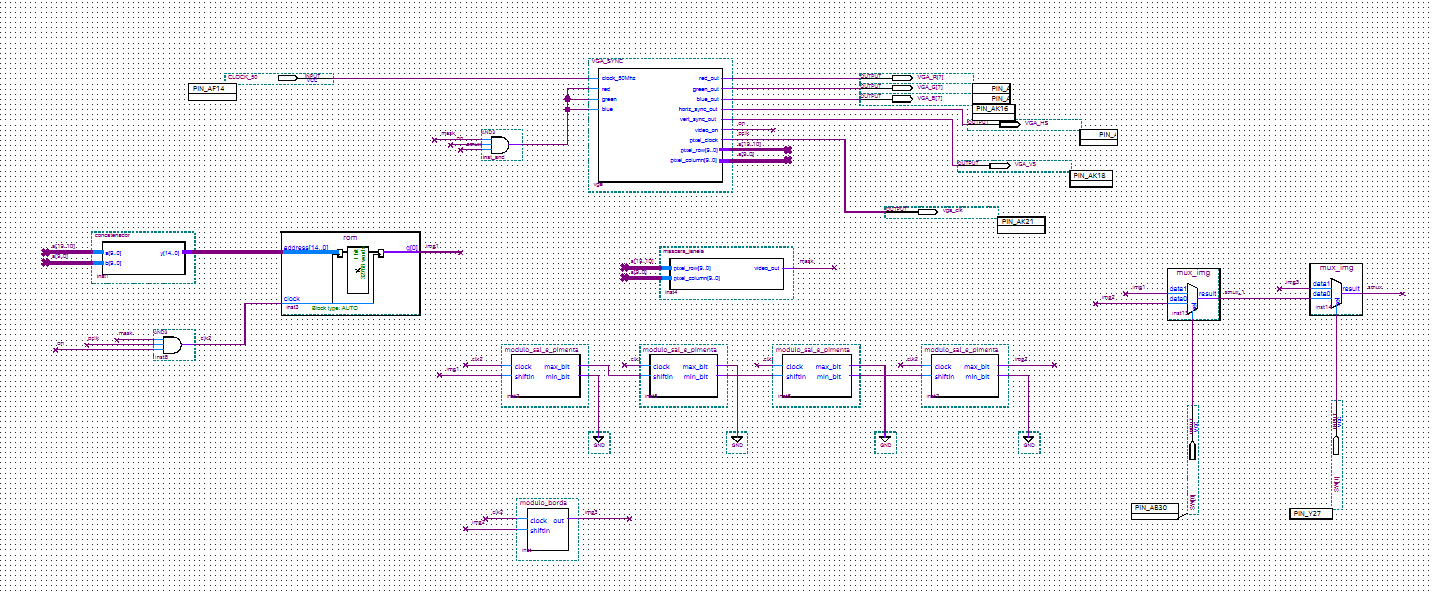
\includegraphics[width=1.0\textwidth]{vga_filtro_bdf.png}
		\caption{Diagrama BDF do módulo \textit{top-level} \texttt{vga\_filtro} no
			Quartus Prime, mostrando a interligação de todos os componentes do
			sistema.}
		\label{fig:vga_filtro_bdf}
	\end{figure}
	
	Os módulos principais são, em ordem de fluxo de dados:
	
	\begin{itemize}
		\item \texttt{VGA\_SYNC} --- Controlador VGA fornecido; gera \texttt{HSync},
		\texttt{VSync}, \texttt{video\_on}, \texttt{pixel\_clock} e os contadores
		de coordenadas \texttt{pixel\_column}/\texttt{pixel\_row};
		\item \texttt{concatenador} --- Concatena os contadores de linha e coluna do
		VGA para formar o endereço de 15 bits da ROM;
		\item \texttt{rom} --- Memória ROM com a imagem binária ruidosa 256$\times$128;
		\item \texttt{modulo\_sal\_e\_pimenta} --- Módulo de filtragem morfológica
		(erosão ou dilatação), instanciado 4 vezes em cascata;
		\item \texttt{modulo\_borda} --- Módulo de detecção de bordas;
		\item \texttt{mascara\_janela} --- Módulo de mascaramento da região VGA;
		\item \texttt{mux\_img} --- Multiplexador de seleção de imagem (2 instâncias).
	\end{itemize}
	
	\subsection{Módulo \texttt{rom} --- Memória da Imagem Binária}
	
	A imagem binária ruidosa de 256$\times$128 pixels é armazenada em uma ROM
	síncrona (\texttt{rom}) inicializada com o arquivo \texttt{.mif} fornecido pelo
	professor. O endereçamento é gerado pelo módulo \texttt{concatenador}, que
	combina os contadores de linha (\texttt{pixel\_row[6:0]}, 7 bits para 0--127)
	e coluna (\texttt{pixel\_column[7:0]}, 8 bits para 0--255) do controlador VGA
	em um endereço linear de 15 bits, totalizando $2^{15} = 32.768$ posições de
	1 bit cada. A ROM opera com clock \texttt{clk2} (pixel clock condicionado ao
	mascaramento), de modo que apenas leituras dentro da região de interesse
	avançam o pipeline.
	
	A Figura~\ref{fig:rom_bdf} mostra o diagrama BDF da ROM, gerado no Quartus Prime.
	
	\begin{figure}[H]
		\centering
		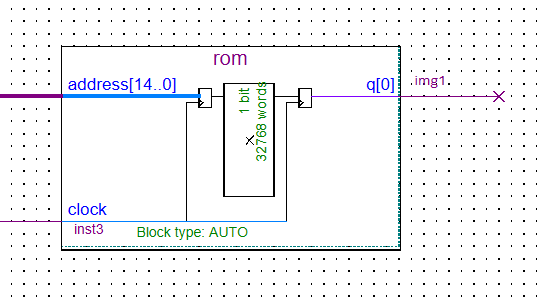
\includegraphics[width=0.80\textwidth]{rom_bdf.png}
		\caption{Diagrama BDF do módulo \texttt{rom} no Quartus Prime, evidenciando
			as entradas de clock e endereço e a saída de dado de 1 bit.}
		\label{fig:rom_bdf}
	\end{figure}
	
	\subsection{Módulo \texttt{max\_min\_9bits} --- Cálculo de Máximo e Mínimo}
	
	O módulo \texttt{max\_min\_9bits} recebe os 9 pixels da janela $3\times3$
	organizados em três vetores de 3 bits (\texttt{in1}, \texttt{in2}, \texttt{in3}),
	concatena-os em um único vetor de 9 bits e percorre todos os bits para determinar
	o máximo e o mínimo. Para pixels binários, esta operação é equivalente a uma
	porta OR de 9 entradas (máximo) e uma porta AND de 9 entradas (mínimo).
	
	\begin{lstlisting}[style=verilog, caption={\texttt{max\_min\_9bits.v} --- Cálculo combinacional de máximo e mínimo sobre janela 3×3 binária.}, label={lst:max_min}]
		module max_min_9bits (
		input  [2:0] in1,
		input  [2:0] in2,
		input  [2:0] in3,
		output reg max_bit,
		output reg min_bit
		);
		integer i;
		reg [8:0] all_bits;
		always @(*) begin
		// Concatenar todos os bits em um unico vetor
		all_bits = {in1, in2, in3};
		// Inicializacao com o primeiro bit
		max_bit = all_bits[0];
		min_bit = all_bits[0];
		// Percorrer os 9 bits para determinar max e min
		for (i = 1; i < 9; i = i + 1) begin
		if (all_bits[i] > max_bit)
		max_bit = all_bits[i];
		if (all_bits[i] < min_bit)
		min_bit = all_bits[i];
		end
		end
		endmodule
	\end{lstlisting}
	
	O bloco \texttt{always @(*)} é puramente combinacional: qualquer alteração nas
	entradas propaga imediatamente para as saídas. O sintetizador do Quartus Prime
	reconhece o laço \texttt{for} com limites estáticos e o expande em lógica
	paralela, produzindo um circuito de dois níveis lógicos sem qualquer sequencial.
	
	\subsection{Módulo \texttt{modulo\_sal\_e\_pimenta} --- Estágio de Pipeline Morfológico}
	
	O módulo \texttt{modulo\_sal\_e\_pimenta} é o componente central do pipeline de
	filtragem. Ele instancia internamente dois registradores de deslocamento de 256
	bits (\texttt{shift\_register}), um registrador de 3 bits (\texttt{shift\_3}) e
	o módulo \texttt{max\_min\_9bits}, formando um estágio completo de filtragem
	morfológica com janela $3\times3$.
	
	\begin{lstlisting}[style=verilog, caption={\texttt{modulo\_sal\_e\_pimenta.v} --- Estágio de pipeline morfológico com line buffers e cálculo de máximo/mínimo.}, label={lst:modulo_sp}]
		module modulo_sal_e_pimenta(
		clock,
		shiftin,
		max_bit,
		min_bit
		);
		input wire  clock;
		input wire  shiftin;
		output wire max_bit;
		output wire min_bit;
		
		wire [255:0] q1;   // line buffer: linha anterior (256 bits)
		wire [255:0] q2;   // line buffer: linha 2 atras  (256 bits)
		wire [2:0]   q3;   // shift_3: 3 pixels mais recentes
		
		// Primeiro line buffer: armazena linha anterior
		shift_register b2v_inst(
		.clock(clock),
		.shiftin(shiftin),
		.q(q1));
		
		// Segundo line buffer: armazena linha 2 atras
		shift_register b2v_inst1(
		.clock(clock),
		.shiftin(q1[0]),
		.q(q2));
		
		// Calculo de maximo e minimo sobre janela 3x3
		max_min_9bits b2v_inst2(
		.in1(q1[255:253]),   // linha anterior: colunas x, x-1, x-2
		.in2(q2[255:253]),   // linha 2 atras:  colunas x, x-1, x-2
		.in3(q3),            // linha corrente: 3 pixels recentes
		.max_bit(max_bit),
		.min_bit(min_bit));
		
		// Registrador de 3 bits: pixels mais recentes da linha corrente
		shift_3 b2v_inst5(
		.clock(clock),
		.shiftin(q2[0]),
		.q(q3));
		
		endmodule
	\end{lstlisting}
	
	Este módulo é instanciado 4 vezes em cascata no \textit{top-level}
	\texttt{vga\_filtro}, com a saída de cada instância alimentando a entrada da
	seguinte, conforme a sequência erosão $\to$ dilatação $\to$ dilatação $\to$ erosão
	descrita na Seção~2.1. As instâncias e suas funções no pipeline são:
	
	\begin{table}[H]
		\centering
		\caption{Instâncias do módulo \texttt{modulo\_sal\_e\_pimenta} e suas
			funções no pipeline morfológico.}
		\label{tab:instancias}
		\begin{tabular}{llll}
			\toprule
			\textbf{Instância} & \textbf{Entrada}              & \textbf{Saída usada}          & \textbf{Operação} \\
			\midrule
			\texttt{b2v\_inst2} & \texttt{img1} (ROM)          & \texttt{min\_bit} (WIRE\_1)   & Erosão (mínimo)   \\
			\texttt{b2v\_inst5} & \texttt{WIRE\_1}             & \texttt{min\_bit} (WIRE\_2)   & Dilatação (máximo)\\
			\texttt{b2v\_inst6} & \texttt{WIRE\_2}             & \texttt{min\_bit} (WIRE\_3)   & Dilatação (máximo)\\
			\texttt{b2v\_inst7} & \texttt{WIRE\_3}             & \texttt{max\_bit} (img2)      & Erosão (mínimo)   \\
			\bottomrule
		\end{tabular}
	\end{table}
	
	\noindent Observa-se que as instâncias \texttt{b2v\_inst2} e \texttt{b2v\_inst6}
	utilizam a saída \texttt{min\_bit} (erosão) e as instâncias \texttt{b2v\_inst5}
	e \texttt{b2v\_inst7} utilizam \texttt{max\_bit} (dilatação), implementando a
	sequência abertura + fechamento.
	
	\subsection{Módulo \texttt{modulo\_borda} e \texttt{edge\_detector\_3x3} --- Detector de Bordas (Parte 2)}
	
	O módulo \texttt{edge\_detector\_3x3} implementa a detecção de bordas por XOR
	entre o pixel central e seus 8 vizinhos. A saída é $1$ se qualquer vizinho
	diferir do pixel central, indicando que o pixel central está em uma região de
	transição.
	
	\begin{lstlisting}[style=verilog, caption={\texttt{edge\_detector\_3x3.v} --- Detector de bordas combinacional por XOR com o pixel central.}, label={lst:edge}]
		module edge_detector_3x3 (
		input  [2:0] in1,  // linha superior: P1 P2 P3
		input  [2:0] in2,  // linha central:  P4 P5 P6
		input  [2:0] in3,  // linha inferior: P7 P8 P9
		output       out
		);
		wire p1 = in1[0];
		wire p2 = in1[1];
		wire p3 = in1[2];
		wire p4 = in2[0];
		wire p5 = in2[1]; // pixel central
		wire p6 = in2[2];
		wire p7 = in3[0];
		wire p8 = in3[1];
		wire p9 = in3[2];
		
		// XOR de cada vizinho com o pixel central
		wire e1 = p5 ^ p1;
		wire e2 = p5 ^ p2;
		wire e3 = p5 ^ p3;
		wire e4 = p5 ^ p4;
		wire e6 = p5 ^ p6;
		wire e7 = p5 ^ p7;
		wire e8 = p5 ^ p8;
		wire e9 = p5 ^ p9;
		
		// Borda ativada se qualquer vizinho diferir do centro
		assign out = e1 | e2 | e3 | e4 | e6 | e7 | e8 | e9;
		endmodule
	\end{lstlisting}
	
	O módulo \texttt{modulo\_borda} encapsula o \texttt{edge\_detector\_3x3} com a
	mesma estrutura de \textit{line buffers} do \texttt{modulo\_sal\_e\_pimenta},
	substituindo o \texttt{max\_min\_9bits} pelo detector de bordas e expondo apenas
	a saída \texttt{out}. Isso garante que o módulo de borda seja inserido no
	pipeline VGA com a mesma interface e a mesma latência de sincronismo dos demais
	módulos.
	
	No \textit{top-level} \texttt{vga\_filtro}, a saída \texttt{img3} do
	\texttt{modulo\_borda} recebe como entrada \texttt{img2} (imagem já filtrada pelo
	pipeline morfológico de 4 estágios), de forma que a detecção de bordas opera
	sobre a imagem \textit{após} a remoção de ruído, produzindo bordas mais limpas
	e sem artefatos.
	
	\subsection{Módulo \texttt{mascara\_janela} --- Mascaramento da Região VGA}
	
	O módulo \texttt{mascara\_janela} verifica se as coordenadas de varredura atuais
	(\texttt{pixel\_column}, \texttt{pixel\_row}) estão dentro da região de interesse
	(coluna $< 256$ e linha $< 128$). Quando dentro da região, a saída \texttt{video\_out}
	é $1$; fora, é $0$, apagando o pixel correspondente. Esta saída é usada de duas
	formas no \textit{top-level}:
	
	\begin{itemize}
		\item Como fator do clock do pipeline: \texttt{clk2 = mask \& pclk \& on},
		garantindo que o pipeline avance apenas quando o VGA está varrendo a
		região da imagem;
		\item Como fator da saída RGB: \texttt{SYNTHESIZED\_WIRE\_7 = mask \& on \& smux},
		apagando a tela fora da região de interesse.
	\end{itemize}
	
	\subsection{Módulo \texttt{mux\_img} --- Seleção de Imagem por Chave}
	
	O módulo \texttt{mux\_img} é um multiplexador 2:1 simples:
	
	\begin{itemize}
		\item Primeira instância (\texttt{b2v\_inst13}): seleciona entre a imagem
		original \texttt{img1} (\texttt{data0}) e a imagem filtrada \texttt{img2}
		(\texttt{data1}), controlada por \texttt{SW[0]};
		\item Segunda instância (\texttt{b2v\_inst14}): seleciona entre a saída da
		primeira instância (\texttt{data0}) e a imagem com bordas \texttt{img3}
		(\texttt{data1}), controlada por \texttt{SW[1]}.
	\end{itemize}
	
	A combinação das duas chaves oferece três modos de visualização:
	
	\begin{table}[H]
		\centering
		\caption{Modos de visualização selecionáveis pelas chaves da placa DE1.}
		\label{tab:modos}
		\begin{tabular}{ccl}
			\toprule
			\textbf{SW[1]} & \textbf{SW[0]} & \textbf{Imagem exibida} \\
			\midrule
			0 & 0 & Original (ruidosa)      \\
			0 & 1 & Filtrada (sem ruído)    \\
			1 & X & Bordas detectadas       \\
			\bottomrule
		\end{tabular}
	\end{table}
	
	\subsection{Módulo \textit{Top-Level} \texttt{vga\_filtro}}
	
	O módulo \texttt{vga\_filtro} interliga todos os componentes descritos acima.
	Sua interface expõe apenas os sinais físicos da placa DE1: clock de 50~MHz
	(\texttt{CLOCK\_50}), chaves (\texttt{SW[1:0]}), saídas VGA (\texttt{VGA\_HS},
	\texttt{VGA\_VS}, \texttt{VGA\_R}, \texttt{VGA\_G}, \texttt{VGA\_B}) e o
	clock de pixel (\texttt{vga\_clk}).
	
	\begin{lstlisting}[style=verilog, caption={\texttt{vga\_filtro.v} --- Módulo \textit{top-level} gerado pelo editor BDF do Quartus Prime.}, label={lst:top}]
		module vga_filtro(
		CLOCK_50,
		SW,
		VGA_HS,
		VGA_VS,
		vga_clk,
		VGA_B,
		VGA_G,
		VGA_R
		);
		input  wire        CLOCK_50;
		input  wire [1:0]  SW;
		output wire        VGA_HS;
		output wire        VGA_VS;
		output wire        vga_clk;
		output wire [7:7]  VGA_B;
		output wire [7:7]  VGA_G;
		output wire [7:7]  VGA_R;
		
		// Fios internos
		wire [19:0] a;           // {pixel_row, pixel_column} do VGA
		wire        clk2;        // clock condicionado ao mascaramento
		wire        img1;        // pixel original da ROM
		wire        img2;        // pixel filtrado (saida do pipeline)
		wire        img3;        // pixel com bordas detectadas
		wire        mask;        // sinal de mascaramento de regiao
		wire        on;          // video_on do controlador VGA
		wire        pclk;        // pixel clock do controlador VGA
		wire        smux;        // saida final do mux de selecao
		wire        smux_1;      // saida intermediaria do mux
		wire [14:0] SYNTHESIZED_WIRE_0;   // endereco da ROM
		wire        SYNTHESIZED_WIRE_1;   // apos 1a erosao
		wire        SYNTHESIZED_WIRE_2;   // apos 1a dilatacao
		wire        SYNTHESIZED_WIRE_3;   // apos 2a dilatacao
		wire        SYNTHESIZED_WIRE_7;   // pixel RGB final
		
		// Detector de bordas (Parte 2)
		modulo_borda b2v_inst(
		.clock(clk2),
		.shiftin(img2),
		.out(img3));
		
		// Concatenador de enderecos: {row, column} -> ROM address
		concatenador b2v_inst1(
		.a(a[19:10]),
		.b(a[9:0]),
		.y(SYNTHESIZED_WIRE_0));
		
		// Mux 1: original vs filtrado (SW[0])
		mux_img b2v_inst13(
		.data1(img1),
		.data0(img2),
		.sel(SW[0]),
		.result(smux_1));
		
		// Mux 2: (original/filtrado) vs bordas (SW[1])
		mux_img b2v_inst14(
		.data1(img3),
		.data0(smux_1),
		.sel(SW[1]),
		.result(smux));
		
		// Estagio 1: Erosao (retira sal)
		modulo_sal_e_pimenta b2v_inst2(
		.clock(clk2),
		.shiftin(img1),
		.max_bit(SYNTHESIZED_WIRE_1));
		
		// ROM de imagem binaria ruidosa
		rom b2v_inst3(
		.clock(clk2),
		.address(SYNTHESIZED_WIRE_0),
		.q(img1));
		
		// Modulo de mascaramento 256x128
		mascara_janela b2v_inst4(
		.pixel_column(a[9:0]),
		.pixel_row(a[19:10]),
		.video_out(mask));
		
		// Estagio 2: Dilatacao (restaura bordas apos erosao)
		modulo_sal_e_pimenta b2v_inst5(
		.clock(clk2),
		.shiftin(SYNTHESIZED_WIRE_1),
		.min_bit(SYNTHESIZED_WIRE_2));
		
		// Estagio 3: Dilatacao (retira pimenta)
		modulo_sal_e_pimenta b2v_inst6(
		.clock(clk2),
		.shiftin(SYNTHESIZED_WIRE_2),
		.min_bit(SYNTHESIZED_WIRE_3));
		
		// Estagio 4: Erosao (restaura bordas apos dilatacao)
		modulo_sal_e_pimenta b2v_inst7(
		.clock(clk2),
		.shiftin(SYNTHESIZED_WIRE_3),
		.max_bit(img2));
		
		// Clock do pipeline: ativo apenas na regiao de interesse
		assign clk2 = mask & pclk & on;
		
		// Sinal RGB final: mascarado e selecionado
		assign SYNTHESIZED_WIRE_7 = mask & on & smux;
		
		// Controlador VGA (VHDL, fornecido pelo professor)
		VGA_SYNC b2v_vga(
		.clock_50Mhz(CLOCK_50),
		.red(SYNTHESIZED_WIRE_7),
		.green(SYNTHESIZED_WIRE_7),
		.blue(SYNTHESIZED_WIRE_7),
		.red_out(VGA_R),
		.green_out(VGA_G),
		.blue_out(VGA_B),
		.horiz_sync_out(VGA_HS),
		.vert_sync_out(VGA_VS),
		.video_on(on),
		.pixel_clock(pclk),
		.pixel_column(a[9:0]),
		.pixel_row(a[19:10]));
		
		assign vga_clk = pclk;
		
		endmodule
	\end{lstlisting}
	
	% ============================================================
	%  SEÇÃO 4 — DISCUSSÃO DOS RESULTADOS
	% ============================================================
	\section{Discussão dos Resultados}
	
	\subsection{Eficácia da Filtragem Morfológica}
	
	A cadeia de quatro estágios morfológicos encadeados --- erosão, dilatação,
	dilatação, erosão --- implementa corretamente a sequência abertura + fechamento
	sobre a imagem binária ruidosa. A abertura (estágios 1 e 2) elimina os pixels
	brancos isolados de sal: a erosão do primeiro estágio apaga qualquer pixel branco
	cujos 8 vizinhos não sejam todos brancos, e a dilatação do segundo estágio
	restaura as bordas das regiões brancas maiores que não foram afetadas pela erosão.
	O fechamento (estágios 3 e 4) opera de forma simétrica sobre os pixels pretos
	isolados de pimenta.
	
	A Figura~\ref{fig:img_ruido} apresenta a imagem binária original com ruído sal e
	pimenta, tal como armazenada na ROM e exibida no monitor VGA com \texttt{SW[1:0] = 00}.
	São visíveis os pixels brancos espúrios em regiões escuras (sal) e os pixels pretos
	espúrios em regiões claras (pimenta), distribuídos aleatoriamente por toda a imagem.
	
	\begin{figure}[H]
		\centering
		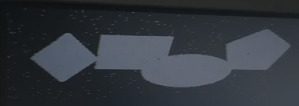
\includegraphics[width=0.75\textwidth]{image_with_noise.jpeg}
		\caption{Imagem binária original com ruído sal e pimenta exibida no monitor VGA
			(\texttt{SW[1:0] = 00}). Pixels espúrios brancos e pretos são claramente
			visíveis distribuídos pela imagem.}
		\label{fig:img_ruido}
	\end{figure}
	
	A Figura~\ref{fig:img_filtrada} apresenta a imagem após o processamento pelo
	pipeline morfológico de quatro estágios (\texttt{SW[1:0] = 01}). A comparação
	direta com a Figura~\ref{fig:img_ruido} evidencia a remoção efetiva dos pixels
	espúrios, com as estruturas binárias originais preservadas. Pixels isolados de
	sal e pimenta foram eliminados sem degradação perceptível das bordas das regiões.
	
	\begin{figure}[H]
		\centering
		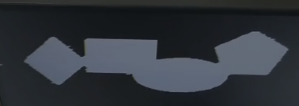
\includegraphics[width=0.75\textwidth]{image_filtered_no_noise.jpeg}
		\caption{Imagem binária após filtragem morfológica pela sequência abertura +
			fechamento (\texttt{SW[1:0] = 01}). O ruído sal e pimenta foi removido com
			preservação das estruturas originais.}
		\label{fig:img_filtrada}
	\end{figure}
	
	O resultado observável no monitor VGA confirma que a qualidade da filtragem é
	função direta do tamanho do elemento estruturante: o quadrado $3\times3$ é eficaz
	para ruído de amplitude 1 pixel, mas insuficiente para clusters de ruído com mais
	de 1 pixel de extensão.
	
	\subsection{Sincronismo entre Pipeline e Varredura VGA}
	
	A estratégia de condicionar o clock do pipeline (\texttt{clk2 = mask \& pclk \& on})
	ao sinal de mascaramento e ao \texttt{video\_on} do controlador VGA é uma solução
	elegante para o problema de sincronismo. O pipeline avança exatamente no mesmo
	ritmo que a varredura VGA percorre a região de interesse, garantindo que o pixel
	processado na saída do pipeline corresponda sempre ao pixel sendo exibido no
	monitor.
	
	Esta abordagem dispensa qualquer lógica de controle de fluxo adicional
	(\textit{handshaking}, FIFOs ou contadores externos), simplificando
	significativamente o projeto e tornando a latência do pipeline transparente para
	o sistema VGA. A desvantagem é que o pipeline fica ocioso durante os períodos
	de \textit{blanking} horizontal e vertical, mas isso não afeta a correção do
	resultado.
	
	\subsection{Seleção de Visualização por Chaves}
	
	O esquema de dois multiplexadores encadeados (\texttt{mux\_img}) controlados por
	\texttt{SW[0]} e \texttt{SW[1]} oferece três modos de visualização com uma
	implementação mínima. A prioridade de \texttt{SW[1]} sobre \texttt{SW[0]} (quando
	\texttt{SW[1] = 1}, \texttt{SW[0]} é irrelevante) é uma característica da
	topologia cascata escolhida, e deve ser documentada ao usuário da placa para
	evitar confusão.
	
	\subsection{Detector de Bordas (Parte 2)}
	
	A detecção de bordas por XOR com o pixel central, implementada no módulo
	\texttt{edge\_detector\_3x3}, produz o contorno de 1 pixel de espessura das
	regiões binárias. Por operar sobre a saída \texttt{img2} (imagem já filtrada),
	as bordas detectadas não são contaminadas por ruído residual.
	
	A Figura~\ref{fig:img_bordas} apresenta o resultado da detecção de bordas
	morfológica exibido no monitor VGA (\texttt{SW[1] = 1}). As bordas obtidas
	apresentam espessura de 1 pixel e delineiam com precisão os contornos das
	regiões binárias da imagem filtrada, sem artefatos provenientes do ruído
	original.
	
	\begin{figure}[H]
		\centering
		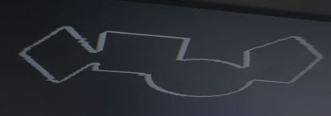
\includegraphics[width=0.75\textwidth]{image_only_borders.jpeg}
		\caption{Resultado da detecção de bordas morfológica sobre a imagem filtrada,
			exibido no monitor VGA (\texttt{SW[1] = 1}). Bordas de 1 pixel de espessura
			delineiam os contornos das regiões binárias sem contaminação por ruído.}
		\label{fig:img_bordas}
	\end{figure}
	
	A implementação é puramente combinacional e reutiliza integralmente a infraestrutura de
	\textit{line buffers} do pipeline existente, adicionando custo negligenciável
	de recursos à síntese.
	
	A formulação por XOR com o pixel central é matematicamente equivalente ao
	gradiente morfológico para imagens binárias (Equação~\ref{eq:borda_xor}),
	mas é computacionalmente mais direta: em vez de calcular explicitamente a
	dilatação e a erosão separadas para então combiná-las por XOR, o módulo
	compara diretamente cada vizinho com o centro, reduzindo o número de operações
	de 18 (9 para max + 9 para min + 1 XOR) para 9 (8 XOR + 1 OR de 8 entradas).
	
	\subsection{Demonstração em Vídeo}
	
	O funcionamento completo do sistema --- incluindo a exibição da imagem ruidosa,
	da imagem filtrada e da detecção de bordas em tempo real na placa DE1 com saída
	VGA --- foi registrado em vídeo e está disponível publicamente no YouTube:
	
	\begin{center}
		\url{https://youtube.com/shorts/RwIUKSUGYYw?feature=share}
	\end{center}
	
	\noindent O vídeo demonstra a alternância entre os três modos de visualização
	por meio das chaves \texttt{SW[0]} e \texttt{SW[1]} da placa, evidenciando o
	funcionamento correto do pipeline morfológico e do detector de bordas em hardware.
	
	% ============================================================
	%  SEÇÃO 5 — CONCLUSÕES
	% ============================================================
	\section{Conclusões}
	
	Esta prática demonstrou com sucesso a implementação de um sistema completo de
	processamento de imagens binárias em FPGA, cobrindo desde o armazenamento da
	imagem em ROM até a exibição do resultado em monitor VGA, passando por uma cadeia
	de filtragem morfológica em pipeline. As principais conclusões são:
	
	\begin{enumerate}
		\item \textbf{Morfologia binária é intrinsecamente eficiente em FPGA:}
		Para pixels de 1 bit, as operações de erosão e dilatação reduzem-se a portas
		AND e OR de 9 entradas, respectivamente. O sintetizador do Quartus Prime
		implementa cada operação em um ou dois níveis lógicos, com frequência de
		operação limitada apenas pela propagação nos registradores de deslocamento.
		Não há necessidade de multiplicadores, somadores ou qualquer aritmética
		além de lógica booleana elementar.
		
		\item \textbf{A estratégia de clock condicionado resolve o sincronismo com
			elegância:} Ao fazer \texttt{clk2 = mask \& pclk \& on}, o pipeline fica
		automaticamente alinhado com a varredura VGA sem nenhuma lógica de controle
		adicional. O pipeline avança exatamente um ciclo por pixel ativo dentro da
		região de interesse, e permanece congelado durante os períodos de
		\textit{blanking}, garantindo que a saída do pipeline corresponda sempre ao
		pixel correto da imagem.
		
		\item \textbf{A arquitetura de line buffers é escalável e reutilizável:}
		O padrão de dois registradores de deslocamento de 256 bits mais um de 3 bits
		foi reutilizado identicamente em todos os estágios do pipeline --- tanto para
		a filtragem morfológica quanto para o detector de bordas. Esta uniformidade
		de interface simplifica a integração no diagrama BDF e facilita a adição de
		novos operadores de processamento no futuro.
		
		\item \textbf{O editor BDF do Quartus Prime é adequado para integração de
			alto nível:} A interligação dos módulos por esquemático, em vez de código
		Verilog estrutural, oferece visibilidade imediata da arquitetura do sistema
		e facilita a identificação de conexões incorretas durante o desenvolvimento.
		Os módulos individuais, desenvolvidos em Verilog, foram instanciados e
		conectados graficamente sem ambiguidade.
		
		\item \textbf{A Parte 2 exemplifica a composibilidade do design morfológico:}
		A adição do detector de bordas ao sistema existente exigiu apenas um novo
		módulo (\texttt{modulo\_borda} com \texttt{edge\_detector\_3x3}) e uma
		instância adicional de \texttt{mux\_img}, sem qualquer modificação nos
		módulos existentes. Isso demonstra que operadores morfológicos compostos
		podem ser construídos de forma incremental sobre a mesma infraestrutura de
		hardware, reduzindo significativamente o esforço de desenvolvimento.
	\end{enumerate}
	
	% ============================================================
	%  SEÇÃO 6 — REFERÊNCIAS BIBLIOGRÁFICAS (ABNT)
	% ============================================================
	\section{Referências Bibliográficas}
	
	\begin{thebibliography}{9}
		
		\bibitem{embarcados1}
		EMBARCADOS.
		\textbf{Controlador VGA --- Parte 1}.
		Disponível em: \url{https://embarcados.com.br/controlador-vga-parte-1/}.
		Acesso em: 25 mai. 2026.
		
		\bibitem{embarcados2}
		EMBARCADOS.
		\textbf{Controlador VGA --- Parte 2}.
		Disponível em: \url{https://embarcados.com.br/controlador-vga-parte-2/}.
		Acesso em: 25 mai. 2026.
		
		\bibitem{pcmag_vga}
		PC MAGAZINE.
		\textbf{VGA (Video Graphics Array)}.
		Disponível em: \url{https://www.pcmag.com/encyclopedia/term/vga}.
		Acesso em: 25 mai. 2026.
		
		\bibitem{gonzalez}
		GONZALEZ, Rafael C.; WOODS, Richard E.
		\textbf{Digital Image Processing}.
		4. ed. New York: Pearson, 2018.
		
		\bibitem{serra}
		SERRA, Jean.
		\textbf{Image Analysis and Mathematical Morphology}.
		London: Academic Press, 1982.
		
		\bibitem{quartus}
		INTEL CORPORATION.
		\textbf{Quartus Prime Standard Edition Handbook}.
		Disponível em: \url{https://www.intel.com/content/www/us/en/programmable/documentation/}.
		Acesso em: 25 mai. 2026.
		
		\bibitem{roteiro5}
		PEDRINO, Emerson Carlos.
		\textbf{Roteiro da Prática 5: Filtro de Máximo/Mínimo em Hardware para
			Processamento de Imagens Binárias}.
		São Carlos: UFSCar --- Departamento de Computação, 2026.
		Disponível em: $\langle$\url{https://ava.ufscar.br}$\rangle$. Acesso em: 25 mai. 2026.
		
		\bibitem{patterson}
		PATTERSON, David A.; HENNESSY, John L.
		\textbf{Organização e Projeto de Computadores: a Interface Hardware/Software}.
		5. ed. Rio de Janeiro: Elsevier, 2017.
		
		\bibitem{thomas}
		THOMAS, Donald E.; MOORBY, Philip R.
		\textbf{The Verilog Hardware Description Language}.
		5. ed. New York: Springer, 2002.
		
	\end{thebibliography}
	
\end{document}